\section{The Thorin functional from the arithmetic}\label{ch:arith}

The Thorin measure has two descriptions: the zeros give its atoms, and the explicit formula gives it from the gamma factor and the primes without reference to any zero. Section~\ref{ch:heat} proves the lower rungs of the positivity ladder with both, the explicit formula near $t=0$ and the zeros away from it, and Section~\ref{ch:finite} shows that no finite set of such tests decides the Thorin condition. Here the arithmetic description is taken on its own, following \cite[Chapter 7]{P26}. Defined as a functional on test functions, the Thorin measure needs no hypothesis on the zeros; Weil's explicit formula identifies it with evaluation at the zeros; and on the heat kernel the primes give the heat trace, losing about $87$ digits to cancellation per unit of $t$.

\subsection{The Thorin functional and the explicit formula}\label{sec:ch14:functional}

The Thorin measure cannot be introduced as a measure without assuming the conclusion. If $W$ were known to be completely monotone, Bernstein's theorem would supply a unique positive measure $U$ with $W(t)=\int e^{-tz}U(dz)$, but complete monotonicity of $W$ is RH. Nor is $\sum_k\delta_{a_k}$ a measure on $[0,\infty)$ unless every $a_k$ is real and nonnegative, which is RH again; an atom at a nonreal $a_k$ can be paired only with functions defined off the real axis. The remedy is to define $U$ as a linear functional on a class of test functions large enough to determine it and small enough that the arithmetic side converges.

Let $\mathcal T$ be the set of functions $\varphi(z)=h(\sqrt z)$ with $h$ even, holomorphic in $|\im r|\le\frac12+c$ for some $c>0$ and $O((1+|r|)^{-2-c})$ there, and let $g(x)=\frac1{2\pi}\int h(r)e^{-irx}dr$. Since $h$ is even, $\varphi$ does not depend on the choice of square root, and it is holomorphic on the image $\{r^2:|\im r|<\frac12+c\}$ of the strip, the region inside a parabola through $-(\frac12+c)^2$, which contains $-\frac14$ and every $a_k$. Define
\begin{equation}\label{eq:ch14:U}
\begin{aligned}
\langle U,\varphi\rangle&=\varphi\Big(-\frac14\Big)+\frac1{4\pi}\int_{\mathbb R}\varphi(r^2)\,m(r)\,dr-\sum_{n\ge2}\frac{\Lambda(n)}{\sqrt n}\,g(\log n),\\
m(r)&=\re\psi\Big(\frac14+\frac{ir}2\Big)-\log\pi ,
\end{aligned}
\end{equation}
where $\psi=\Gamma'/\Gamma$ and $\Lambda$ is the von Mangoldt function. No zero appears in this definition. Weil's explicit formula \cite{Weil52}, \cite[Theorem 5.12]{IwaniecKowalski04} identifies the functional: $\langle U,\varphi\rangle=\sum_k\varphi(a_k)$ for every $\varphi\in\mathcal T$, the sum running over the exponents $a_k=-(\rho_k-\frac12)^2$ of Section~\ref{ch:clock}, one for each pair $\{\rho,1-\rho\}$, and in particular $\langle U,e^{-t\cdot}\rangle=W(t)$ \cite[Proposition 9.4]{P17}.

Each term of \eqref{eq:ch14:U} has its own source. The term $\varphi(-\frac14)=h(\frac i2)$ comes from the poles of $\pi^{-s/2}\Gamma(s/2)\zeta(s)$ at $s=1$ and $s=0$, which the factor $s(s-1)$ of $\xi$ removes; it is the only evaluation of $\varphi$ off $[0,\infty)$, and it is not an atom of $U$ but one of three pieces whose sum is the evaluation at the exponents. The integral is the contribution of the gamma factor: with the Riemann Siegel theta function $\vartheta(r)=\im\log\Gamma(\frac14+\frac{ir}2)-\frac r2\log\pi$ we have $m=2\vartheta'$, so the integral is $\pi^{-1}\int_0^\infty h\,d\vartheta$, the integral of $h$ against the smooth part of the zero counting function. The prime sum is the fluctuating part. The half width $\frac12+c$ of the strip does two things: it makes $g(x)=O(e^{-(1/2+c)|x|})$, so that the prime sum converges absolutely against the weight $n^{-1/2}$, and it contains the ordinates $\pm\frac i2$ of the poles and the complex ordinate $\gamma_k=-i(\rho_k-\frac12)$ of every zero, since $|\im\gamma_k|=|\re\rho_k-\frac12|<\frac12$.

The sine squared lemma \eqref{eq:sin2} rewrites the functional in terms of variograms. By \eqref{eq:ch10:variogram} its kernel carries each $\varphi\in\mathcal T$ to $g(0)-g(x)$, a variogram when $h\ge0$, and the functional takes the absolutely convergent form \cite[Proposition 9.2]{P17}
\begin{multline*}
\langle U,\varphi\rangle=\int_0^\infty\frac{e^{-x/2}}{e^{2x}-1}\big(g(0)-g(x)\big)\,dx-C_\Gamma g(0)\\
+\int_0^\infty e^{x/2}g(x)\,dx-\sum_{n\ge2}\frac{\Lambda(n)}{\sqrt n}g(\log n),
\end{multline*}
where $C_\Gamma=\frac12\log\pi-\frac12\psi(\frac14)-2=0.6860917096$ is the archimedean constant of Section~\ref{sec:ch6:consequences}, equal to $\zeta'(\frac12)/\zeta(\frac12)-2$ because $\xi'(\frac12)=0$. To derive this form, split $\varphi(-\frac14)=\int_0^\infty(e^{x/2}+e^{-x/2})g(x)\,dx$; the half with $e^{-x/2}$ combines with the gamma integral into the first two terms.

This form regularises a formal pairing. Formally $\langle U,\varphi\rangle=\int_0^\infty\big(g(0)-g(x)\big)\,\nu(dx)$, where $\nu$ is the canonical measure of \eqref{eq:split} at $\alpha=\frac12$,
\[
\nu(dx)=\frac{e^{-x/2}\,dx}{e^{2x}-1}-e^{x/2}\,dx+\sum_{n\ge2}\frac{\Lambda(n)}{\sqrt n}\,\delta_{\log n}(dx),
\]
but the pole and prime parts of this pairing diverge through their $g(0)$ terms. Part by part, the absolutely convergent form exceeds the formal pairing by multiples of $g(0)$: by $-C_\Gamma$ for the gamma factor, by $\int_0^\infty e^{x/2}dx$ for the pole and by $-\sum_n\Lambda(n)n^{-1/2}$ for the primes. Continued analytically as in Section~\ref{sec:ch6:consequences}, the last two are $-2$ and $\zeta'(\frac12)/\zeta(\frac12)$, and the three constants cancel by the identity $C_\Gamma+2-\zeta'(\frac12)/\zeta(\frac12)=0$ of that section, which is equivalent to $\xi'(\frac12)=0$. The only negative part of $\nu$ is the pole density $-e^{x/2}dx$, and Section~\ref{sec:ch10:positivity} reads Weil's criterion from this sign pattern. At the basepoint one the pole density is $-dx$, and no analytic continuation is needed there: the prime atoms compensated by the pole density have a convergent sine squared integral, and its convergence is the prime number theorem (Proposition~\ref{bp:prop:sin2}). For $L(s,\chi_{12})$, which has no pole, the prime atoms at the basepoint one carry the signs of $\chi_{12}$ and converge with no compensation (Section~\ref{bp:eta:sec:levy}).

The functional is not in general the limit of the Thorin measures as the basepoint approaches the line. As $\alpha\downarrow\frac12$ the measures $U_\alpha$ of \eqref{eq:Ualpha} converge vaguely to $U_{\rm line}=\sum\delta_{\gamma^2}$, the sum running over the zeros on the line, whatever the truth of RH (Section~\ref{ch:clock} and \cite[Proposition 9.5]{P17}), whereas unconditionally
\[
U=U_{\rm line}+\sum_{a_k\notin(0,\infty)}\delta_{a_k}\quad\text{on }\mathcal T,
\]
the sum running over the nonreal exponents. These come in conjugate pairs $(\gamma-id)^2$ and $(\gamma+id)^2$, one pair for each off line pair $\frac12\pm d+i\gamma$ of Proposition~\ref{prop:struct} (written $\frac12\pm\delta+i\gamma$ there), so $U=U_{\rm line}$ exactly when RH holds \cite[Proposition 9.6]{P17}. The functional evaluates $\varphi$ at both exponents of an off line pair, while in \eqref{eq:struct} the pair contributes kernels $P_{\varepsilon+d}+P_{\varepsilon-d}$ of total mass zero once $\varepsilon<d$, which vanish in the limit. This is why the vague limit in Section~\ref{ch:weak} omits the off line zeros, and why the Thorin mass in Proposition~\ref{prop:zerodensity} misses both members of an off line pair, which produces the factor two there.

\subsection{The heat trace from the primes}\label{sec:ch14:heat}

For $\varphi(z)=e^{-tz}$, that is $h(r)=e^{-tr^2}$ and $g(x)=e^{-x^2/4t}/(2\sqrt{\pi t})$, the functional is the arithmetic form \eqref{eq:ch2:Warith} of the heat trace, $W=\Pi+A-P$, with the polar term $\Pi=e^{t/4}$, the archimedean term $A$ and the prime term $P$ described in Section~\ref{ch:clock}. Table~\ref{tab:ch14:W} extends the comparison of Table~\ref{tab:ch2:W} to smaller and larger $t$. We evaluate the three terms in sixty digit arithmetic, $A$ by adaptive quadrature and $P$ over $n\le2\times10^5$, and compare $\Pi+A-P$ with the sum over the first $1700$ zeros, whose ordinates we take to seventy digits (Appendix~\ref{app:code}); the last column is the number of decimal digits lost to cancellation, $\log_{10}\{(\Pi+|A|+P)/W\}$. The two columns agree to every digit shown.

\begin{table}[htbp]
\centering\footnotesize
\begin{tabular}{@{}rlll@{}}
\toprule
$t$ & polar $\Pi$ & archimedean $A$ & prime $P$\\
\midrule
0.002 & 1.000500 & 0.782881 & $2.6\times10^{-26}$\\
0.005 & 1.001251 & $-0.464059$ & $7.2\times10^{-11}$\\
0.01 & 1.002503 & $-0.852797$ & $8.4\times10^{-6}$\\
0.02 & 1.005013 & $-0.984061$ & 0.002410\\
0.05 & 1.012578 & $-0.954619$ & 0.057914\\
0.1 & 1.025315 & $-0.862510$ & 0.162806\\
0.15 & 1.038212 & $-0.797634$ & 0.240578\\
0.2 & 1.051271 & $-0.749754$ & 0.301517\\
0.3 & 1.077884 & $-0.681852$ & 0.396032\\
\bottomrule
\end{tabular}

\medskip
\begin{tabular}{@{}rlll@{}}
\toprule
$t$ & $\Pi+A-P$ & $W$ from zeros & digits lost\\
\midrule
0.002 & 1.78338120537913 & 1.78338120537913 & 0.0\\
0.005 & 0.537191964091041 & 0.537191964091041 & 0.4\\
0.01 & 0.14969801125378 & 0.14969801125378 & 1.1\\
0.02 & 0.0185412917313195 & 0.0185412917313195 & 2.0\\
0.05 & $4.58783504857357\times10^{-5}$ & $4.58783504857357\times10^{-5}$ & 4.6\\
0.1 & $2.10479979582235\times10^{-9}$ & $2.10479979582235\times10^{-9}$ & 9.0\\
0.15 & $9.65642094572633\times10^{-14}$ & $9.65642094572633\times10^{-14}$ & 13.3\\
0.2 & $4.43018218022364\times10^{-18}$ & $4.43018218022364\times10^{-18}$ & 17.7\\
0.3 & $9.32464654810622\times10^{-27}$ & $9.32464654810622\times10^{-27}$ & 26.4\\
\bottomrule
\end{tabular}
\caption{The heat trace from the explicit formula and from the zeros. For $t\ge0.05$ the digits lost are $\log_{10}2+(\gamma_1^2+\frac14)t/\log10\approx0.30+86.88\,t$.}
\label{tab:ch14:W}
\end{table}

The cancellation follows a simple law. For $t\ge0.005$ the archimedean term is negative (Exercise~\ref{ex:ch14:law}), so $\Pi+|A|+P=2e^{t/4}-W$ and the digits lost are $\log_{10}(2e^{t/4}/W-1)$. Since $W=e^{-\gamma_1^2t}\big(1+O(e^{-(\gamma_2^2-\gamma_1^2)t})\big)$, this is
\[
\log_{10}2+\frac{(\gamma_1^2+\frac14)\,t}{\log10}\approx0.30+86.88\,t
\]
up to an exponentially small error, below $2\times10^{-5}$ for $t\ge0.05$; at $t=0.3$ the law gives $0.30103+26.06294=26.36397$. The intercept $\log_{10}2$ records that $\Pi$ is balanced by $|A|+P$, and the slope exceeds $\gamma_1^2/\log10=86.77$ by $1/(4\log10)$, the growth rate of the polar term (Figure~\ref{fig:ch14:W}).

\begin{figure}[htbp]
\centering
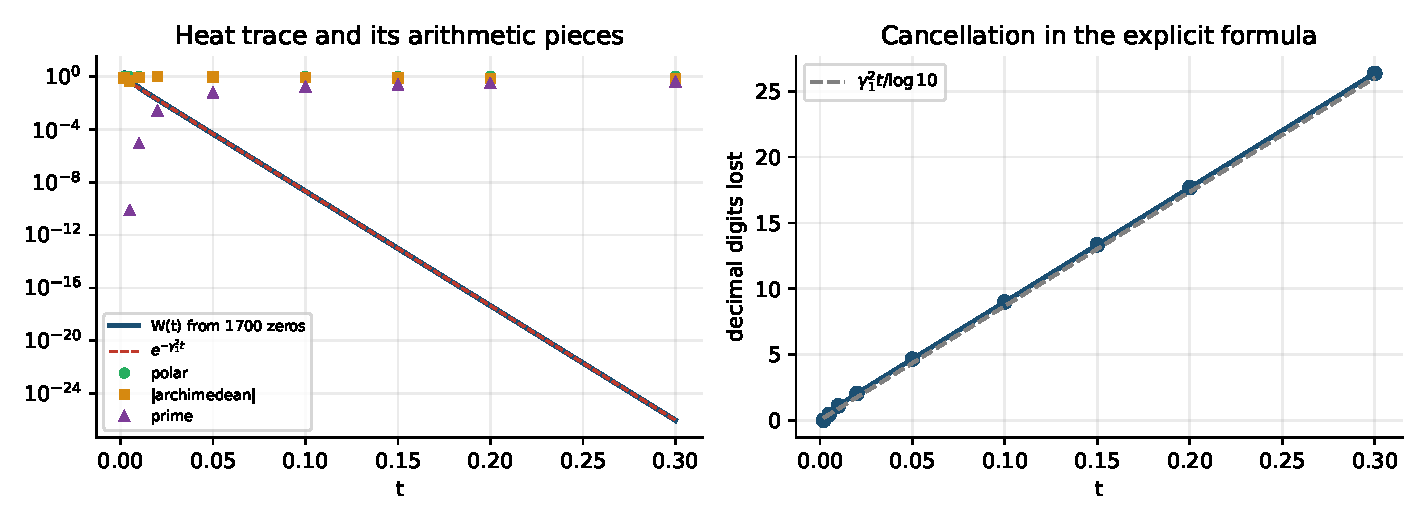
\includegraphics[width=\textwidth]{fig/heattrace.pdf}
\caption{Left: the heat trace from $1700$ zeros, its leading exponential $e^{-\gamma_1^2t}$, and the three arithmetic pieces, the archimedean one in absolute value. Right: digits lost to cancellation in the explicit formula; for $t\ge0.05$ they lie $\log_{10}2+t/(4\log10)$ above the dashed line $\gamma_1^2t/\log10$.}
\label{fig:ch14:W}
\end{figure}

The explicit formula holds exactly, and the cancellation costs working precision and nothing more: $26.4$ digits at $t=0.3$, well within sixty digit arithmetic. It is the price of computing an exponentially small quantity as a difference of terms of size $e^{t/4}$, the price the untilted P\'olya route pays at height $\theta$, where it loses $0.341\,\theta$ digits (Section~\ref{ch:polya}). The zeros give $W$ cheaply at moderate $t$, the primes only near $t=0$. Section~\ref{ch:sato} finds the same profile for the L\'evy density $-W'$ of the subordinator that drives the clock.

The two descriptions divide the work. The arithmetic side is cheap where $g$ is concentrated near $x=0$, so that only small $n$ contribute: at small $t$ for the heat kernel, and only at large resolution for the Poisson kernel $h(r)=P_\varepsilon(\theta-r)+P_\varepsilon(\theta+r)$. That kernel is not in $\mathcal T$, but for $\varepsilon>\frac12$ its transform $g(x)=\pi^{-1}e^{-\varepsilon|x|}\cos\theta x$ makes the prime sum converge absolutely; for smaller $\varepsilon$ the prime side is Selberg's smoothed sum, which with cutoff $X$ uses the primes up to $X^2$ and has error of order $X^{-\varepsilon}/(\varepsilon^2\log X)$ when no zero lies to the right of the critical line, the single zero law of Section~\ref{sec:ch10:selberg}. The spectral side is cheap where the test function is concentrated at the low zeros: at large $t$, and at small $\varepsilon$ on a window. In the proofs of the lower rungs in Section~\ref{ch:heat} the two forms meet at $t=1/20000$, where the inequalities are checked in interval arithmetic. The Thorin condition requires positivity at every scale, and neither side is cheap at every scale. The P\'olya route of Section~\ref{ch:polya} is, but only on a window of finite height, and that restriction is the barrier of Section~\ref{ch:finite}.
